\documentclass{article}
\usepackage{tikz}
\usetikzlibrary{positioning,arrows.meta}
\begin{document}
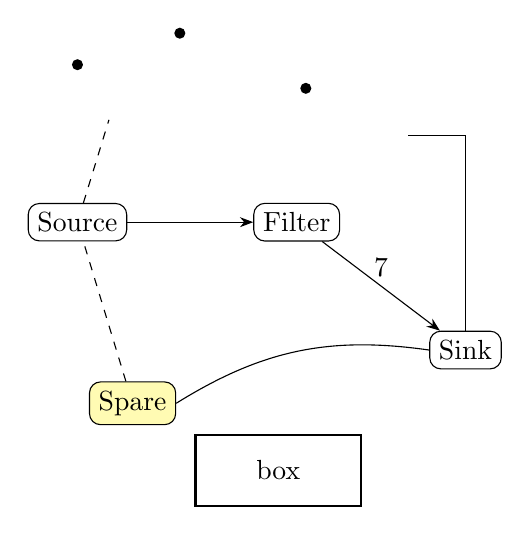
\begin{tikzpicture}[node distance=1.6cm, every node/.style={draw, rounded corners}]
  \node (src) at (0,0) {Source};
  \node[right=of src] (mid) {Filter};
  \node[below right=of mid] (sink) {Sink};
  \node[fill=yellow!30] (aux) at (0.7,-2.3) {Spare};
  \draw[-{Stealth}] (src) -- (mid);
  \draw[-{Stealth}] (mid) -- node[above, draw=none] {7} (sink);
  \draw[dashed] (aux) -- (src) -- ++(0.4,1.3);
  \coordinate (corner) at (4.2,1.1);
  \draw (sink) |- (corner);
  \begin{scope}[shift={(1.5,-3.6)}, line width=0.8pt]
    \draw (0,0) rectangle (2.1,0.9);
    \node[draw=none] at (1.05,0.45) {box};
  \end{scope}
  \foreach \x/\y in {0/2, 1.3/2.4, 2.9/1.7}
    \fill (\x,\y) circle (2pt);
  \draw (aux.east) to[bend left=20] (sink.west);
\end{tikzpicture}
\end{document}
